%% ----------------------------------------------------------------------------
% CVG SA/MA thesis template
%
% Created 03/08/2024 by Tobias Fischer
%% ----------------------------------------------------------------------------

\newpage
\chapter{Related Work}

The related work section has the following purposes: 

\begin{itemize}
 \item \textit{Is the overview concise?} Give an overview of the most relevant work to the needed extent. Make sure the reader can understand your work without referring to other literature.
 \item \textit{Does the compilation of work help to define the ``niche'' you are working in?} Another purpose of this section is to lay the groundwork for showing that you did significant work. The selection and presentation of the related work should enable you to name the implications, differences, and similarities sufficiently in the discussion section.
\end{itemize}

description of task
\section{Visual Question Answering Task (indoor + other)}

VQA vs 3D-QA
OBJECT IDENTIFICATION!!

indoor is a subtask but it is interesting because we can include some 3D element to it
- also this lays the foundation for answering harder questions later on, which cannot be answered simply with 2D methods: eg. about distances and paths, which would be interesting for navigation tasks.
\begin{itemize}
    \item Task description
    \item Expected inputs / outputs
    \item Question ontology
    \item Classical methods (non-SG), strenghts and limitations
    \item Scene Graph methods (Graph Question Answering), strengths and limitations (most of these for indoor scenes say they use graphs but they never utilise edge info)
\end{itemize}

description of data
\section{Scene Graphs}
\begin{itemize}
    \item Scene graph formal definition + advantages
    \item Scene graph generation methods
    \item Graph neural networks
    \item Applications and limitations
\end{itemize}


description of the "building blocks" used to create the model
\section{Image-text pretrained models}

\section{Transformer encoder / decoders}
GNN can be formulated as a 

\section{Datasets}

\textcolor{red}{ScanQA is the only question dataset exclusively about indoor scenes.}
\textcolor{red}{Wrap text around figures?}
\textcolor{red}{Can add this section to 'Related work' instead of an entire independent section.}


\subsection{ScanNet}
\textcolor{red}{add an example of a 3D segmented scene + segmented RGB-D to illustrate what the dataset looks like? can also add to appendix}

The ScanNet dataset consists of 1,513 segmented point clouds of indoor environments, generated from 2,492,518 segmented RGB-D frames. The dataset includes a range of spaces e.g. offices, apartments, bathrooms, libraries, and spans both small spaces and large spaces. The dataset offers both instance-level and semantic-level segmentations. In the following analysis, we only consider the set of ScanNet scenes for which the ScanQA dataset provides question-answer pairs.

In this section, we report some useful dataset statistics for the scenes for which ScanQA question-answer pairs exist.

Figure XX show the type of distribution of scene types.  The three most common scene type are 'Bedroom', 'Living Room' and 'Bathroom'.
\begin{figure}[h!]
    \centering
    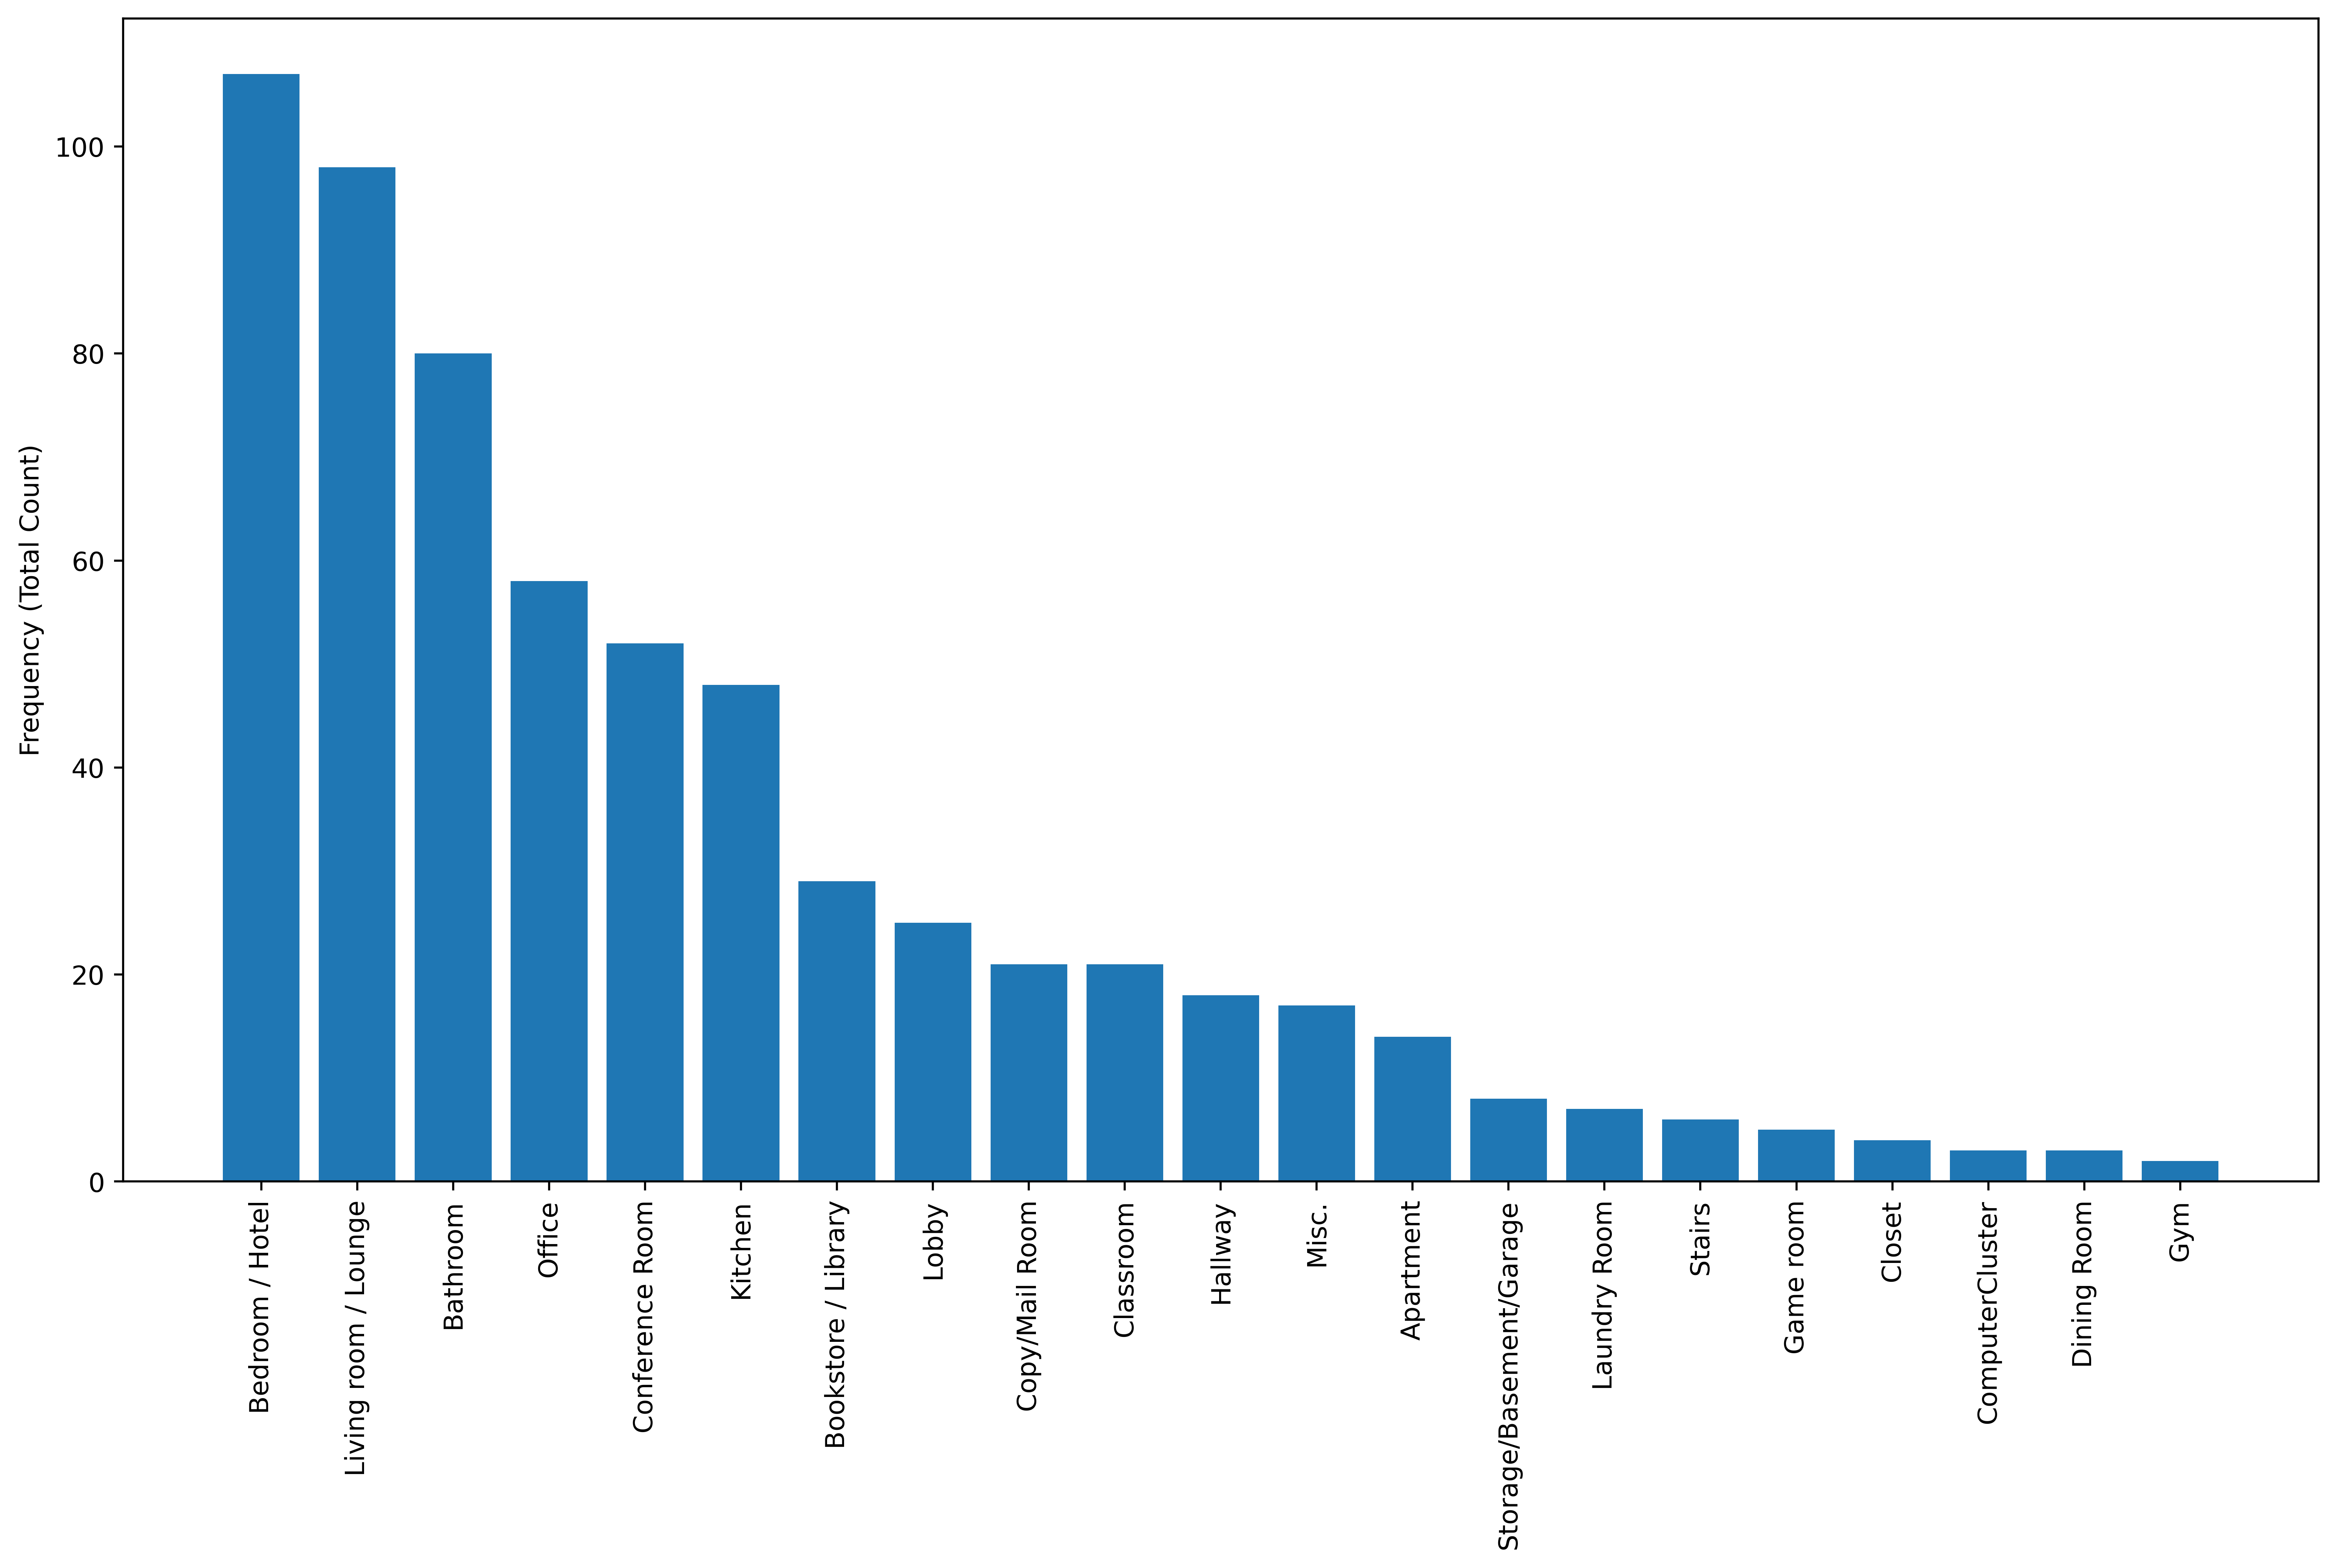
\includegraphics[width=0.5\linewidth]{images/roomtype_frequency.png}
    \caption{Scene type distribution}
    \label{fig:enter-label}
\end{figure}


Figure XX shows the distribution of object labels. We note that the most common label is 'wall' (as all scenes contain multiple walls), followed by 'chair'.
\begin{figure}[h!]
    \centering
    \includegraphics[width=0.5\linewidth]{images/object_frequency.png}
    \caption{Object label distribution \textcolor{red}{remove "other" and add to text instead how many "other" were excluded from the top-30}}
    \label{fig:enter-label}
\end{figure}

\textcolor{red}{+ Avg number of object instances per scene)}


Figure XX shows the inverse object density per scene. This describes how clustered or sparse the scene is. This is a useful metric for understanding how similar we should expect the graphs of ScanSG to be. We note that the object density is fairly consistent across scenes: \textcolor{red}{80$\%$ of scenes have between ... and ... scenes per $m^2$}

\begin{figure}[h!]
    \centering
    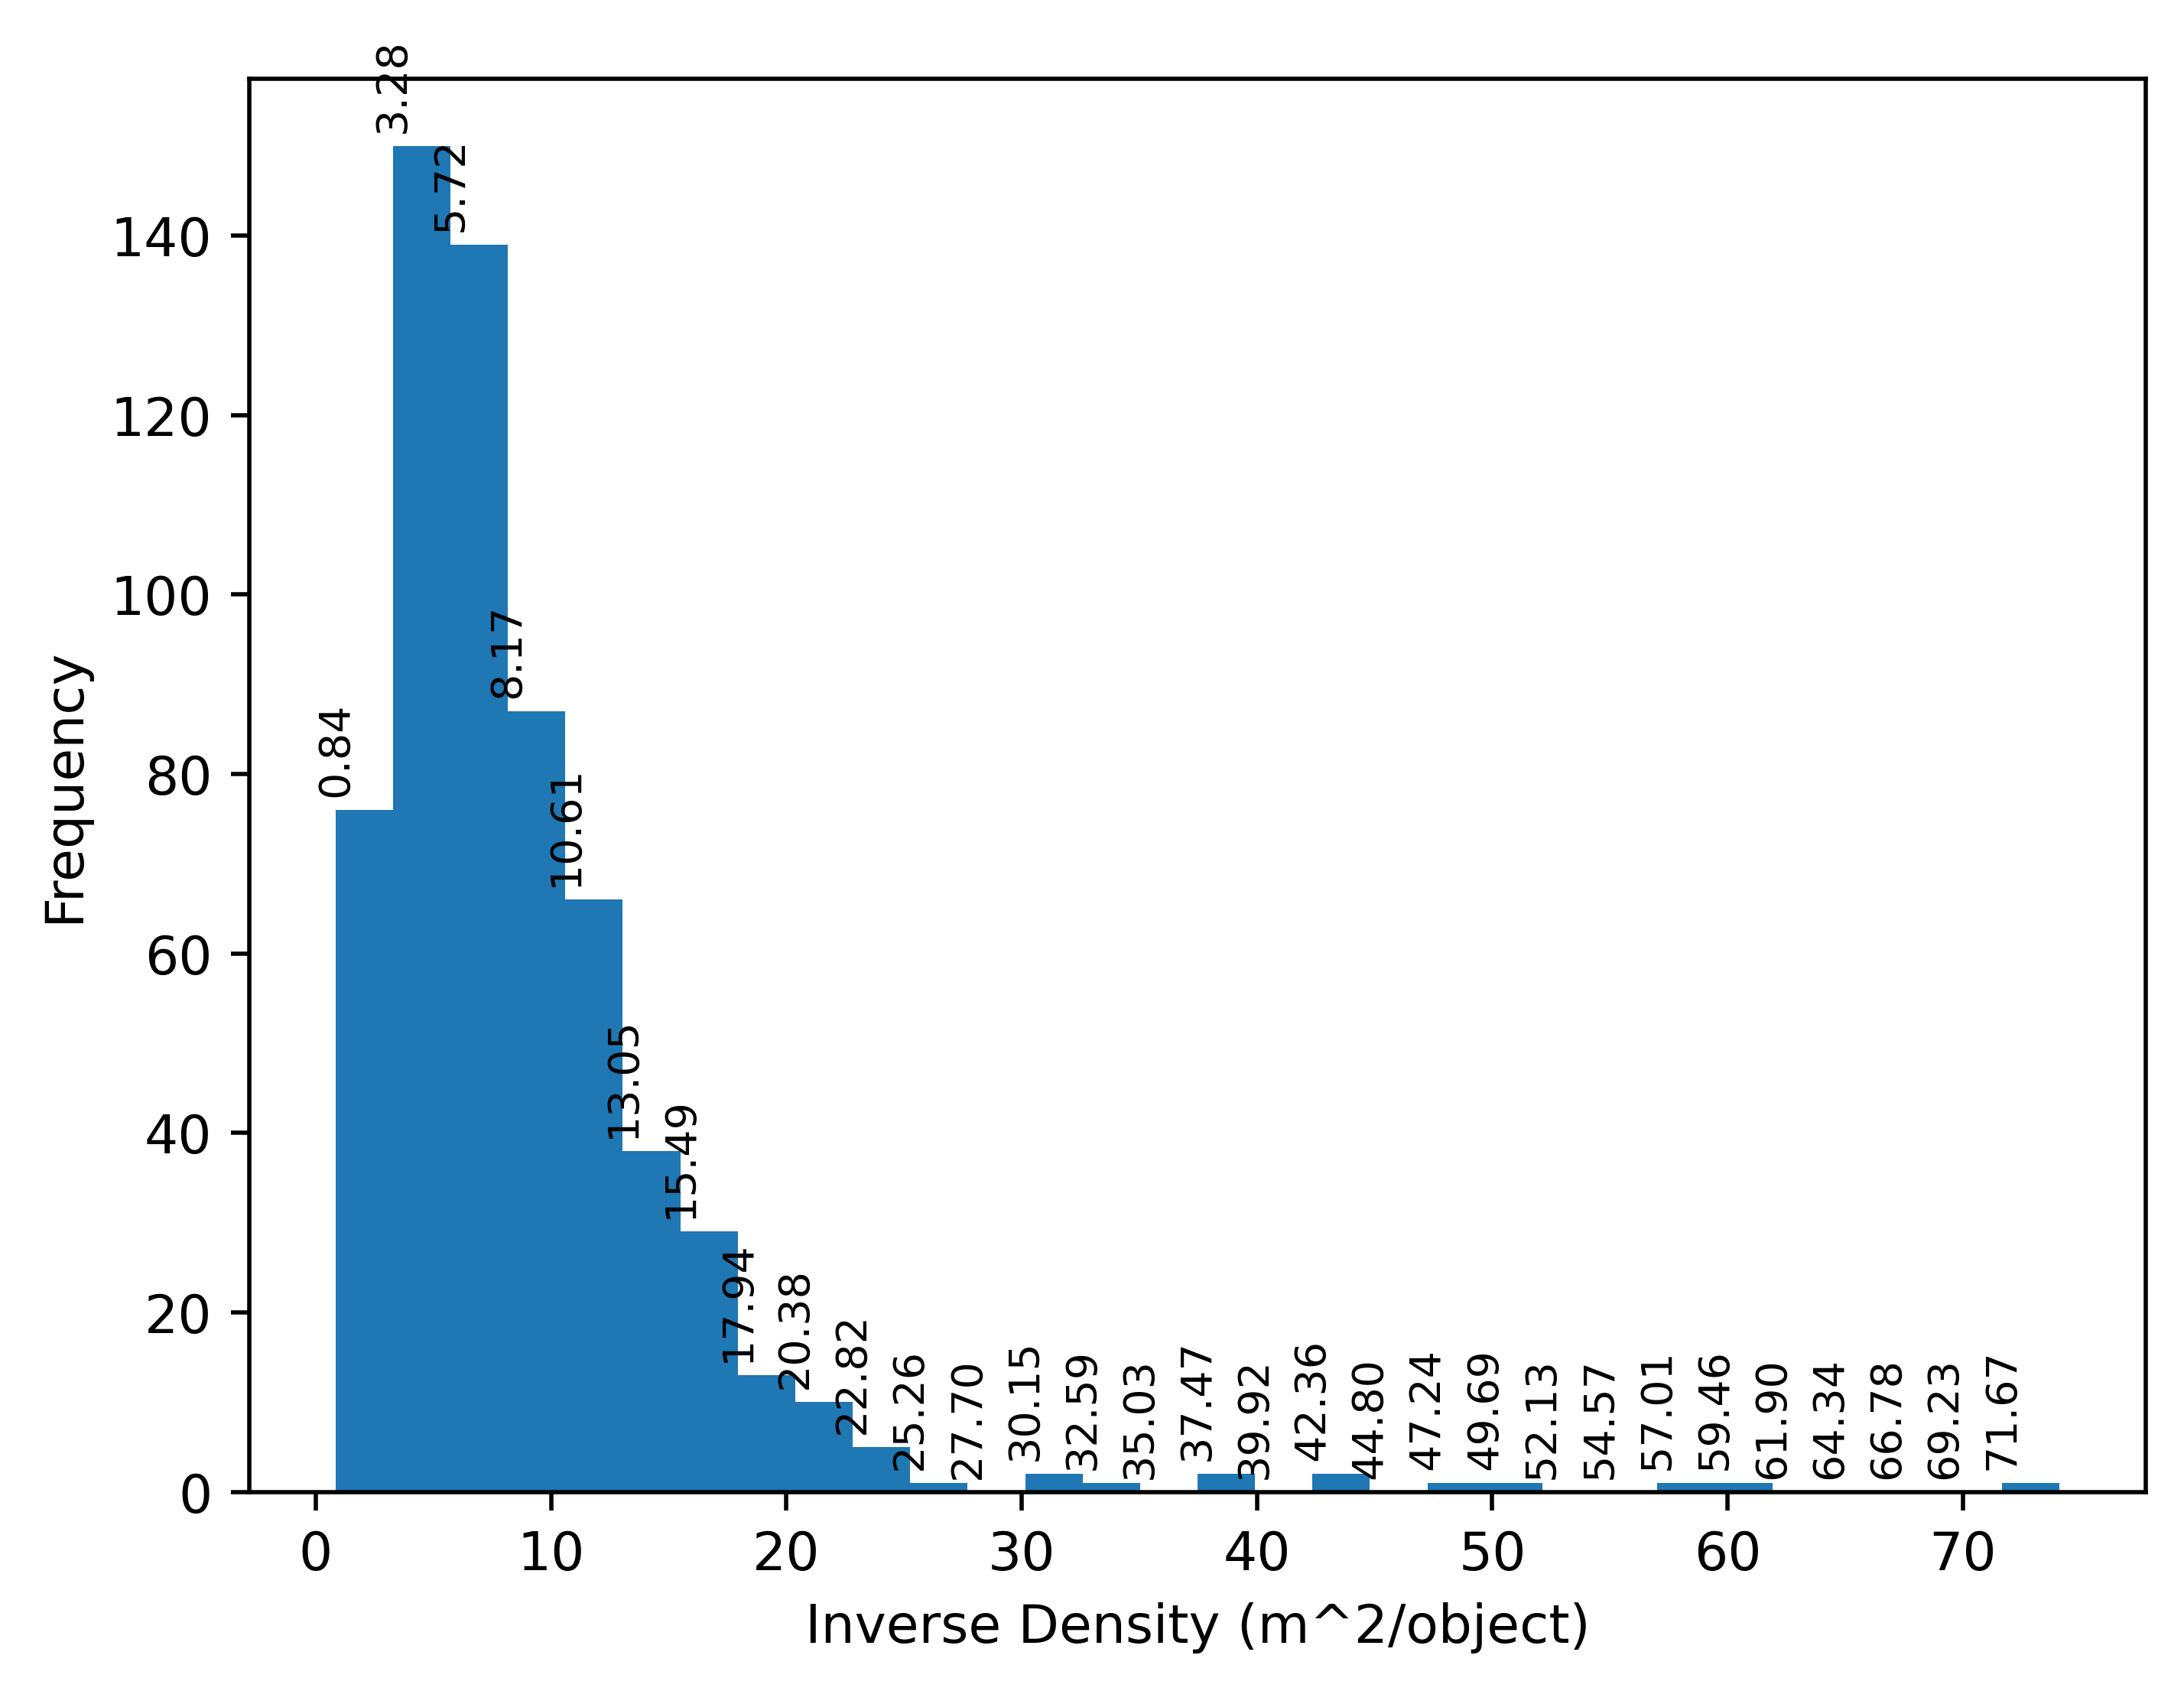
\includegraphics[width=0.5\linewidth]{images/object_density.png}
    \caption{scene density distribution}
    \label{fig:enter-label}
\end{figure}

\subsection{ScanQA}

\textcolor{red}{[Add that each question-answer pair has corresponds to one unique scene, which is specified]}

The ScanQA dataset [XX] consists of 30,238 question-answer pairs about 633 ScanNet scenes. While most questions have a unique answer, some questions have multiple possible answers. To simplify the task at hand, we only consider questions with a unique answer.

\bigskip
\noindent \textbf{Questions}
Sorting out multi-answer entries, we are left with a simplified dataset of 21,324 questions about 632 scenes (on average 33.7 questions per scene). 17,321 of these questions are unique, while 4003 are repeated one or more times. Figure XX shows the most common question types by wording. We note that the most common question phrasings are "What is...", "What color...", "What type..." and "Where is...". These phrasings represent more than half of the dataset. The average question contains 8.8 words.

\begin{figure}[h!]
    \centering
    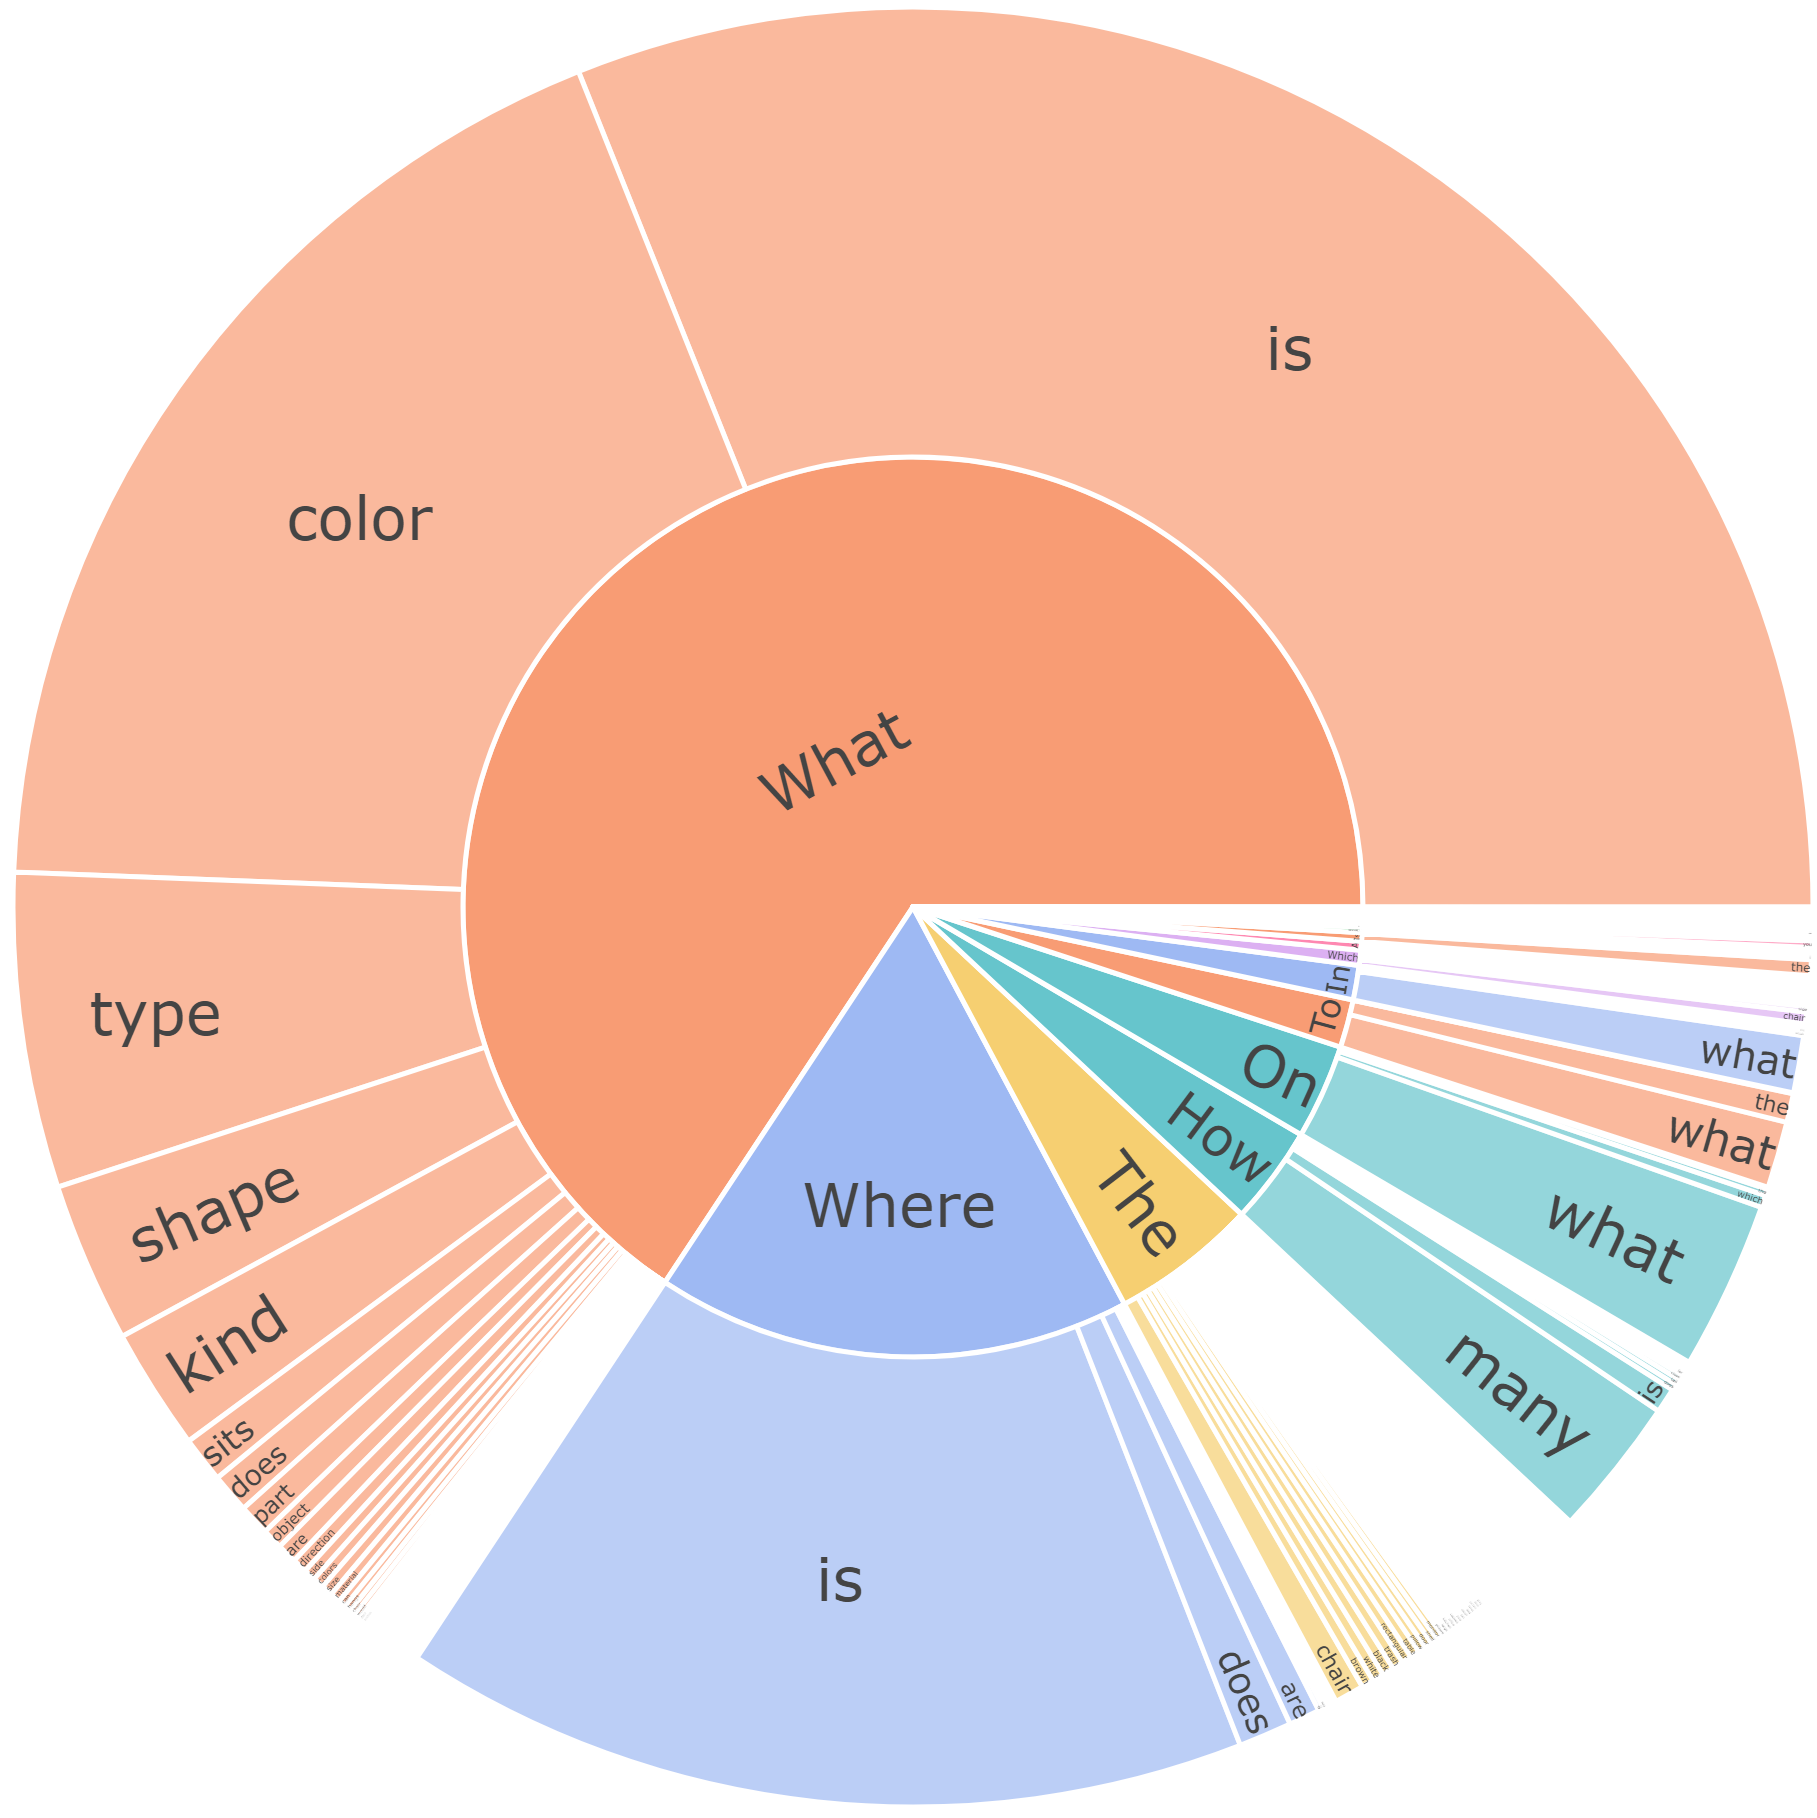
\includegraphics[width=0.5\textwidth]{images/sunburst_high_dpi.png}
    \caption{Most common question types by wording}
    \label{fig:your_label}
\end{figure}


\bigskip
\noindent \textbf{Answers}
The ScanQA dataset provides two types of answers for each question: a long answer, and a short answer. The long answer is a free-form textual answer, while the short answer is simply a single object instance. The short answer can be interpreted as answering "where should one look to answer the question?". In other words, the short answer does not always directly answer the question, but rather specifies the most relevant object in the scene to the question. Table XX provides a few examples of this. We also note that in 61$\%$ of questions, the answer label is directly contained in the question. For example, looking at table XX, the question "What color table is on the left side of the cabinet?" already contains the short answer "table" within the question. In this project, we only consider the short answers, as this allows us to solve the easier and more interpretable task of classification rather than generation.

\begin{table}[h!]
    \centering
    \caption{Examples of long and short answers from the dataset. \bigskip}
    \begin{tabular}{lll}
    \textbf{Question}                                    & \textbf{Long Answer}                & \textbf{Short Answer} \\
    What is in the right corner of room by curtains?     & brown cabinet with tv sitting in it & cabinet               \\
    What color table is on the left side of the cabinet? & light brown                         & table                 \\
    Where is the beige wooden working table placed?      & right of tall cabinet               & cabinet              
    \end{tabular}
\end{table}

\noindent
We note that the quality of question-answer pairs varies, based on the following observations:
\begin{itemize}
    \item Some questions are vague, and do not specify which object instance is referred to. For example, "The trash can is to the left of what?" is unclear, as there are 3 trash cans in the scene and the question does not specify which trash can it is referring to.
    
    \item Some questions have multiple possible answers, but only specify a single answer. For example, the question "What is placed next to the fridge?" has multiple possible answers as many objects are next to the fridge in the scene. However, the answer reported is "door".
    
    \item The short answers provided do not follow a consistent logic: sometimes, the short answer is the subject of the question, while other times it is the object of the question. For example, "Where is the coffee table kept?" is answered by "coffee table" while "What is the coffee table in front of" is answered by "couch" rather than "coffee table".
    
    \item Some questions are poorly phrased, for example "What is the white wooden door?" or have typos, such as "Where is the rectangular keyboard piano lcoared?".
    
    \item Some questions are view dependent, such as "What color table is on the left side of the cabinet?".
\end{itemize}
These observations imply that any model answering the question with a valid but different answer will be penalized as much as if it predicted a completely incorrect answer.

Furthermore, we note that many of the questions do not require much (if any) 3D information to answer. In other words, they could easily be answered only from 2D RGB images. This is likely because the images were generated from the 2D images of the scenes. The dataset contains no questions about distances, paths, dimensions or 3D geometry. 

However, the questions in the dataset are tailored specifically to the ScanNet scenes, and cannot be answered without knowledge of the relevant scene. The dataset does not contain generic questions such as "Where can I watch a film?" but rather scene-specific questions such as "What color towel is on the left of a white towel?".

Figure XX shows the answer distribution in the simplified dataset. We note that the answer distribution is non-uniform, and questions are most commonly answered by the label "chair". 

\begin{figure}[h!]
    \centering
    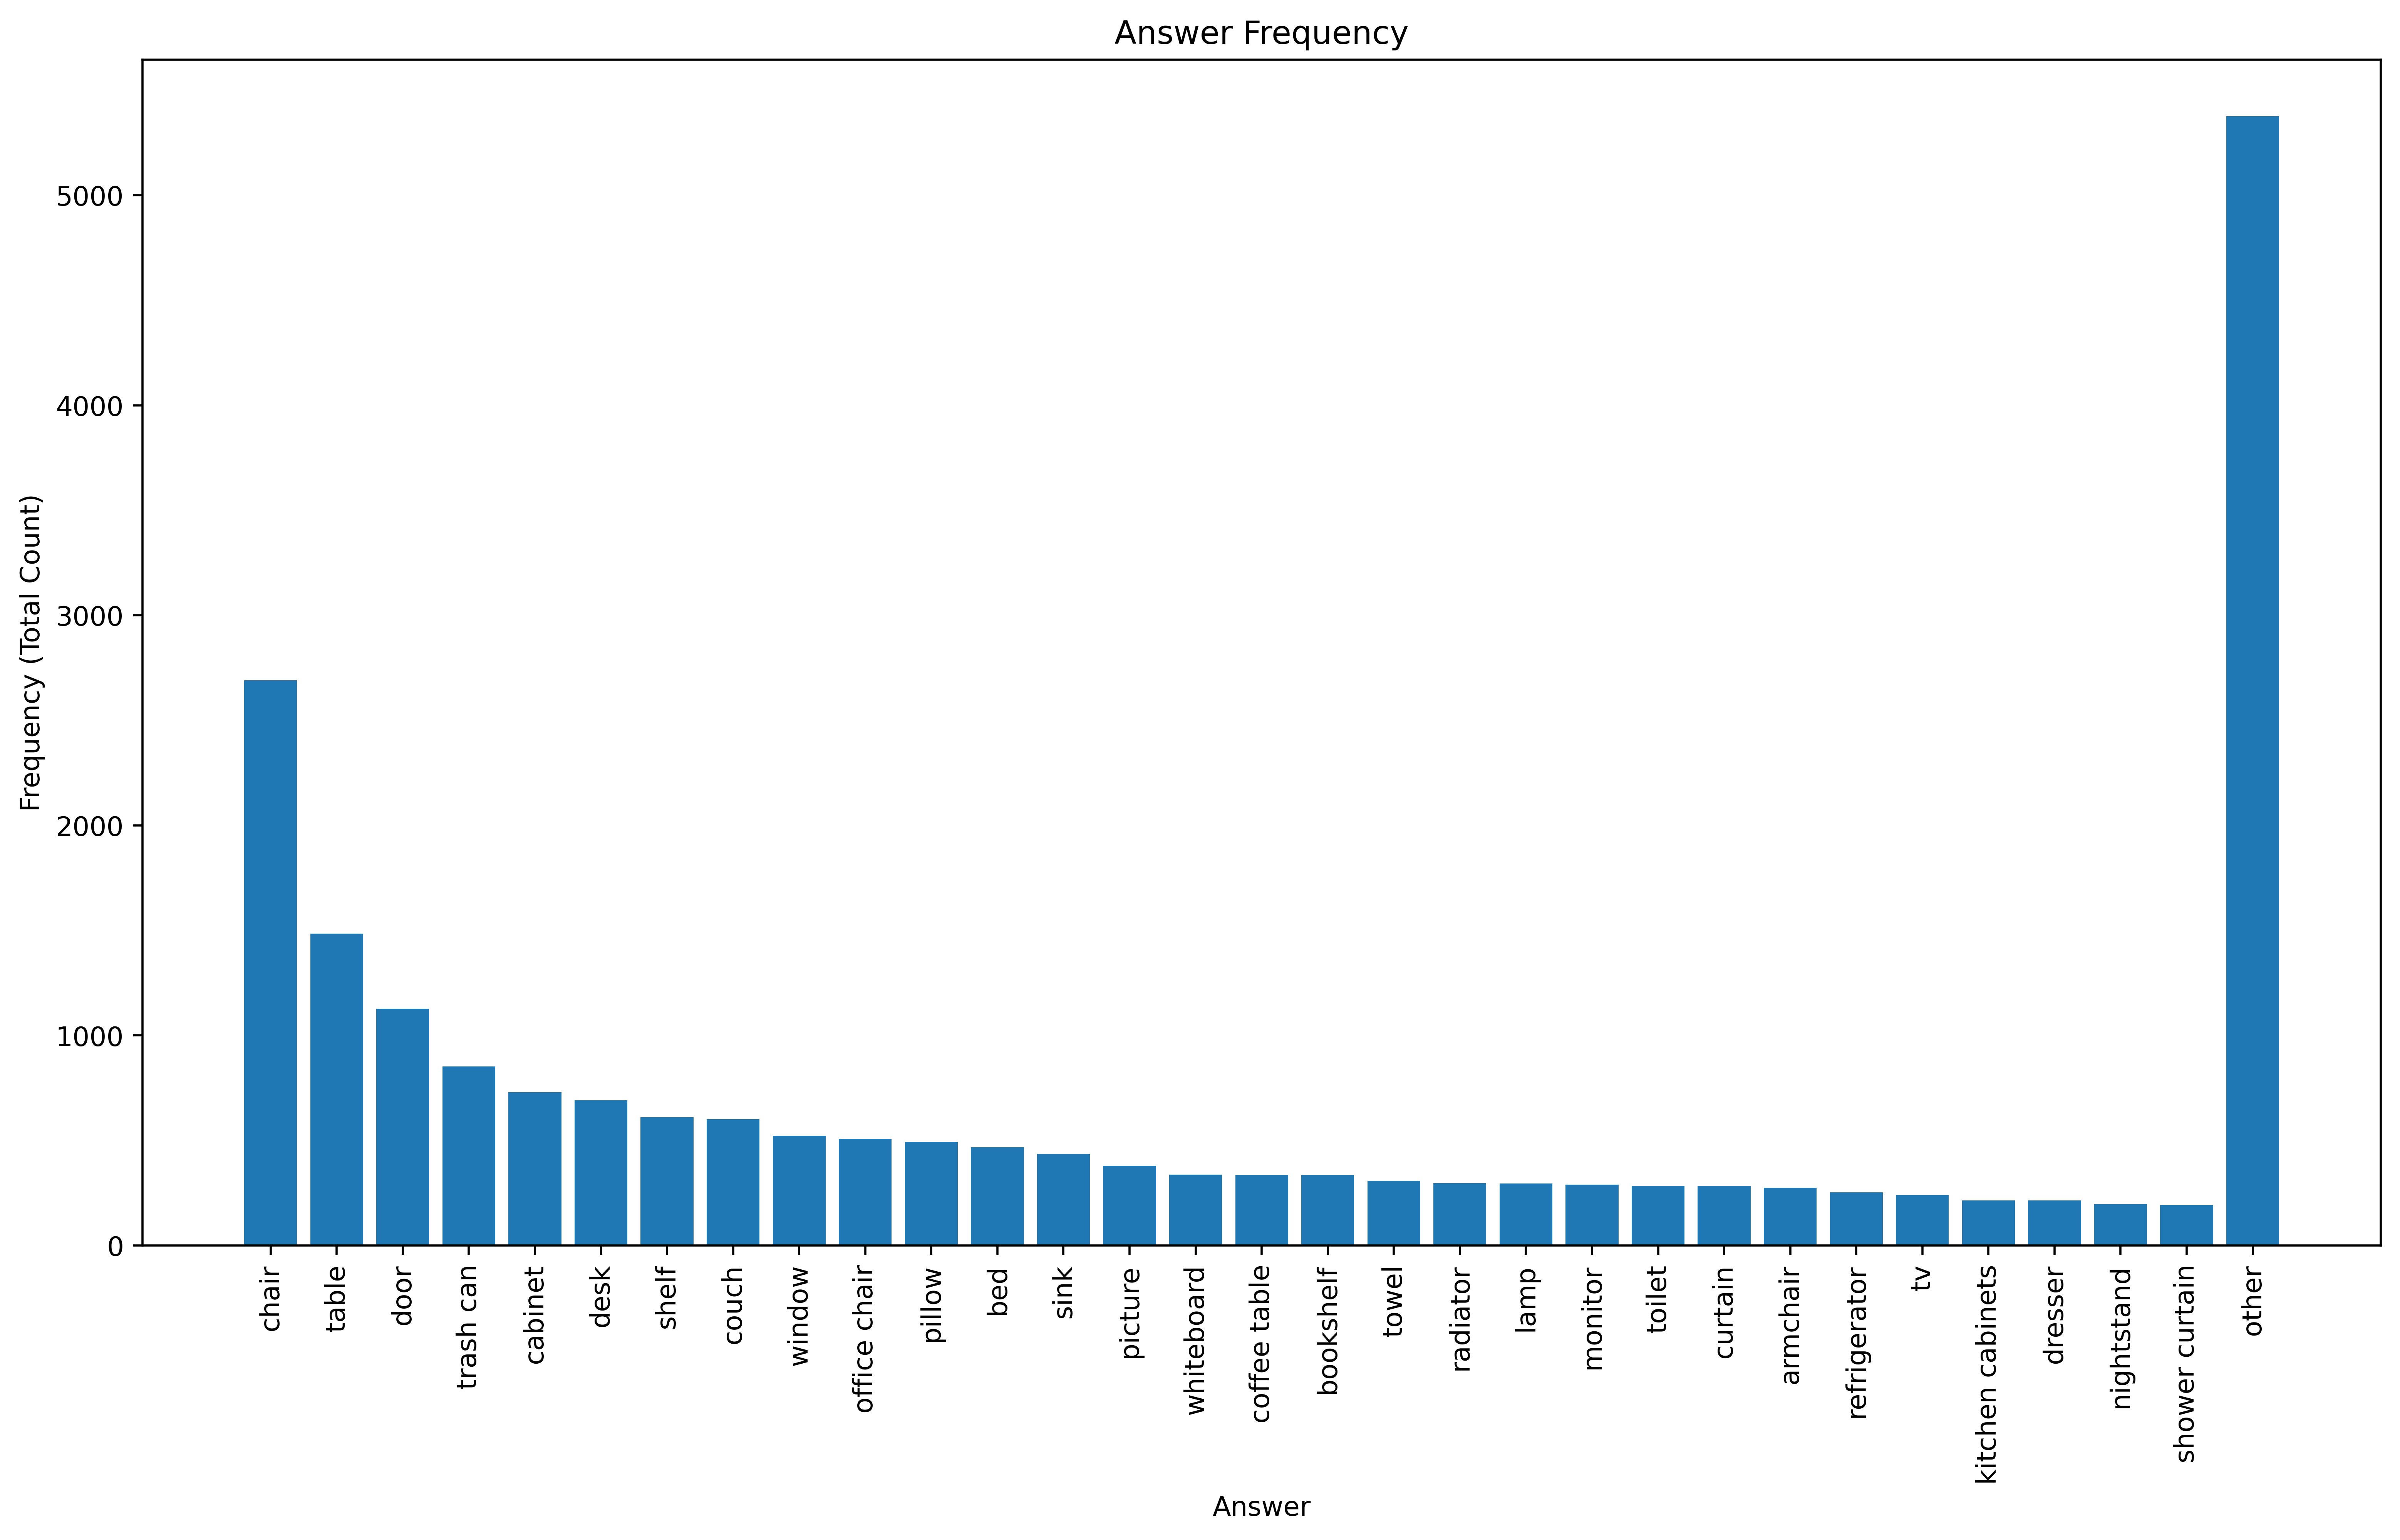
\includegraphics[width=0.5\textwidth]{images/answer_frequency.png}
    \caption{Answer distribution of 30 most common answers. The "other" label groups all other less frequent labels. \textcolor{red}{\textbf{add other(x) with x number of labels contained here, remove title and x-axis title. also make this figure smaller and cleaner and match color scheme to plot above. IMPORTANT: make it vertical instead of horizontal, more pleasant to read in this document}}}
    \label{fig:your_label}
\end{figure}